
\documentclass[handout]{beamer}

\usetheme{Singapore}
\usecolortheme[RGB={0, 32, 91}]{structure}  % Rice blue
\setbeamertemplate{navigation symbols}{\insertframenumber}

\usepackage{ulem}

\title{Probability and Paradoxes in Baseball}
\author{Scott Powers}
\date{}

\begin{document}

  \begin{frame}
    \maketitle
    \begin{center}
      
\includegraphics[width = 2cm]{images/brains_in_a_bar.png}
    \end{center}
  \end{frame}

  \begin{frame}{The Birthday Problem (von Mises, 1939)}
    \begin{itemize}
      \item In a group of $n$ people, what is the probability that at least two will share a birthday?
    \end{itemize}
    \begin{center}
      
\includegraphics[width = 4cm]{images/birthday_cake.jpg}
    \end{center}
    {\bf Q:} How big does $n$ need to be for the probability to exceed 50\%?
    \pause
    {\bf A:} $n \ge 23$
  \end{frame}

  \begin{frame}{Simpson's Paradox (Simpson, 1951)}
    \begin{itemize}
      \item Justice had the higher batting average in 1995 {\it and} 1996,\\but Jeter had the higher combined batting average
    \end{itemize}
    \begin{center}
      \begin{tabular}{l|cc|c}
                      & 1995  & 1996  & Combined\\
                      \hline
        Derek Jeter   & .250  & .314  & .310\\
        David Justice & .253  & .321  & .270
      \end{tabular}
    \end{center}
    {\bf Q:} How is this possible?\\
    \pause
    {\bf A:}
    \begin{center}
      \begin{tabular}{l|cc|c}
                      & 1995  & 1996  & Combined\\
                      \hline
        Derek Jeter   & 12/48   & 183/582 & 195/630\\
        David Justice & 104/411 & 45/140  & 149/551
      \end{tabular}
    \end{center}
  \end{frame}

  \begin{frame}{The Monty Hall Problem (Selman, 1975)}
    \begin{itemize}
      \item On a game show, you are given the choice of three doors
      \begin{itemize}
        \item One door hides a car, and two doors hide a goat
      \end{itemize}
      \item After you choose door \#1, the host opens door \#3, revealing a goat (the host alway reveals a goat behind a different door)
    \end{itemize}
    \begin{center}
      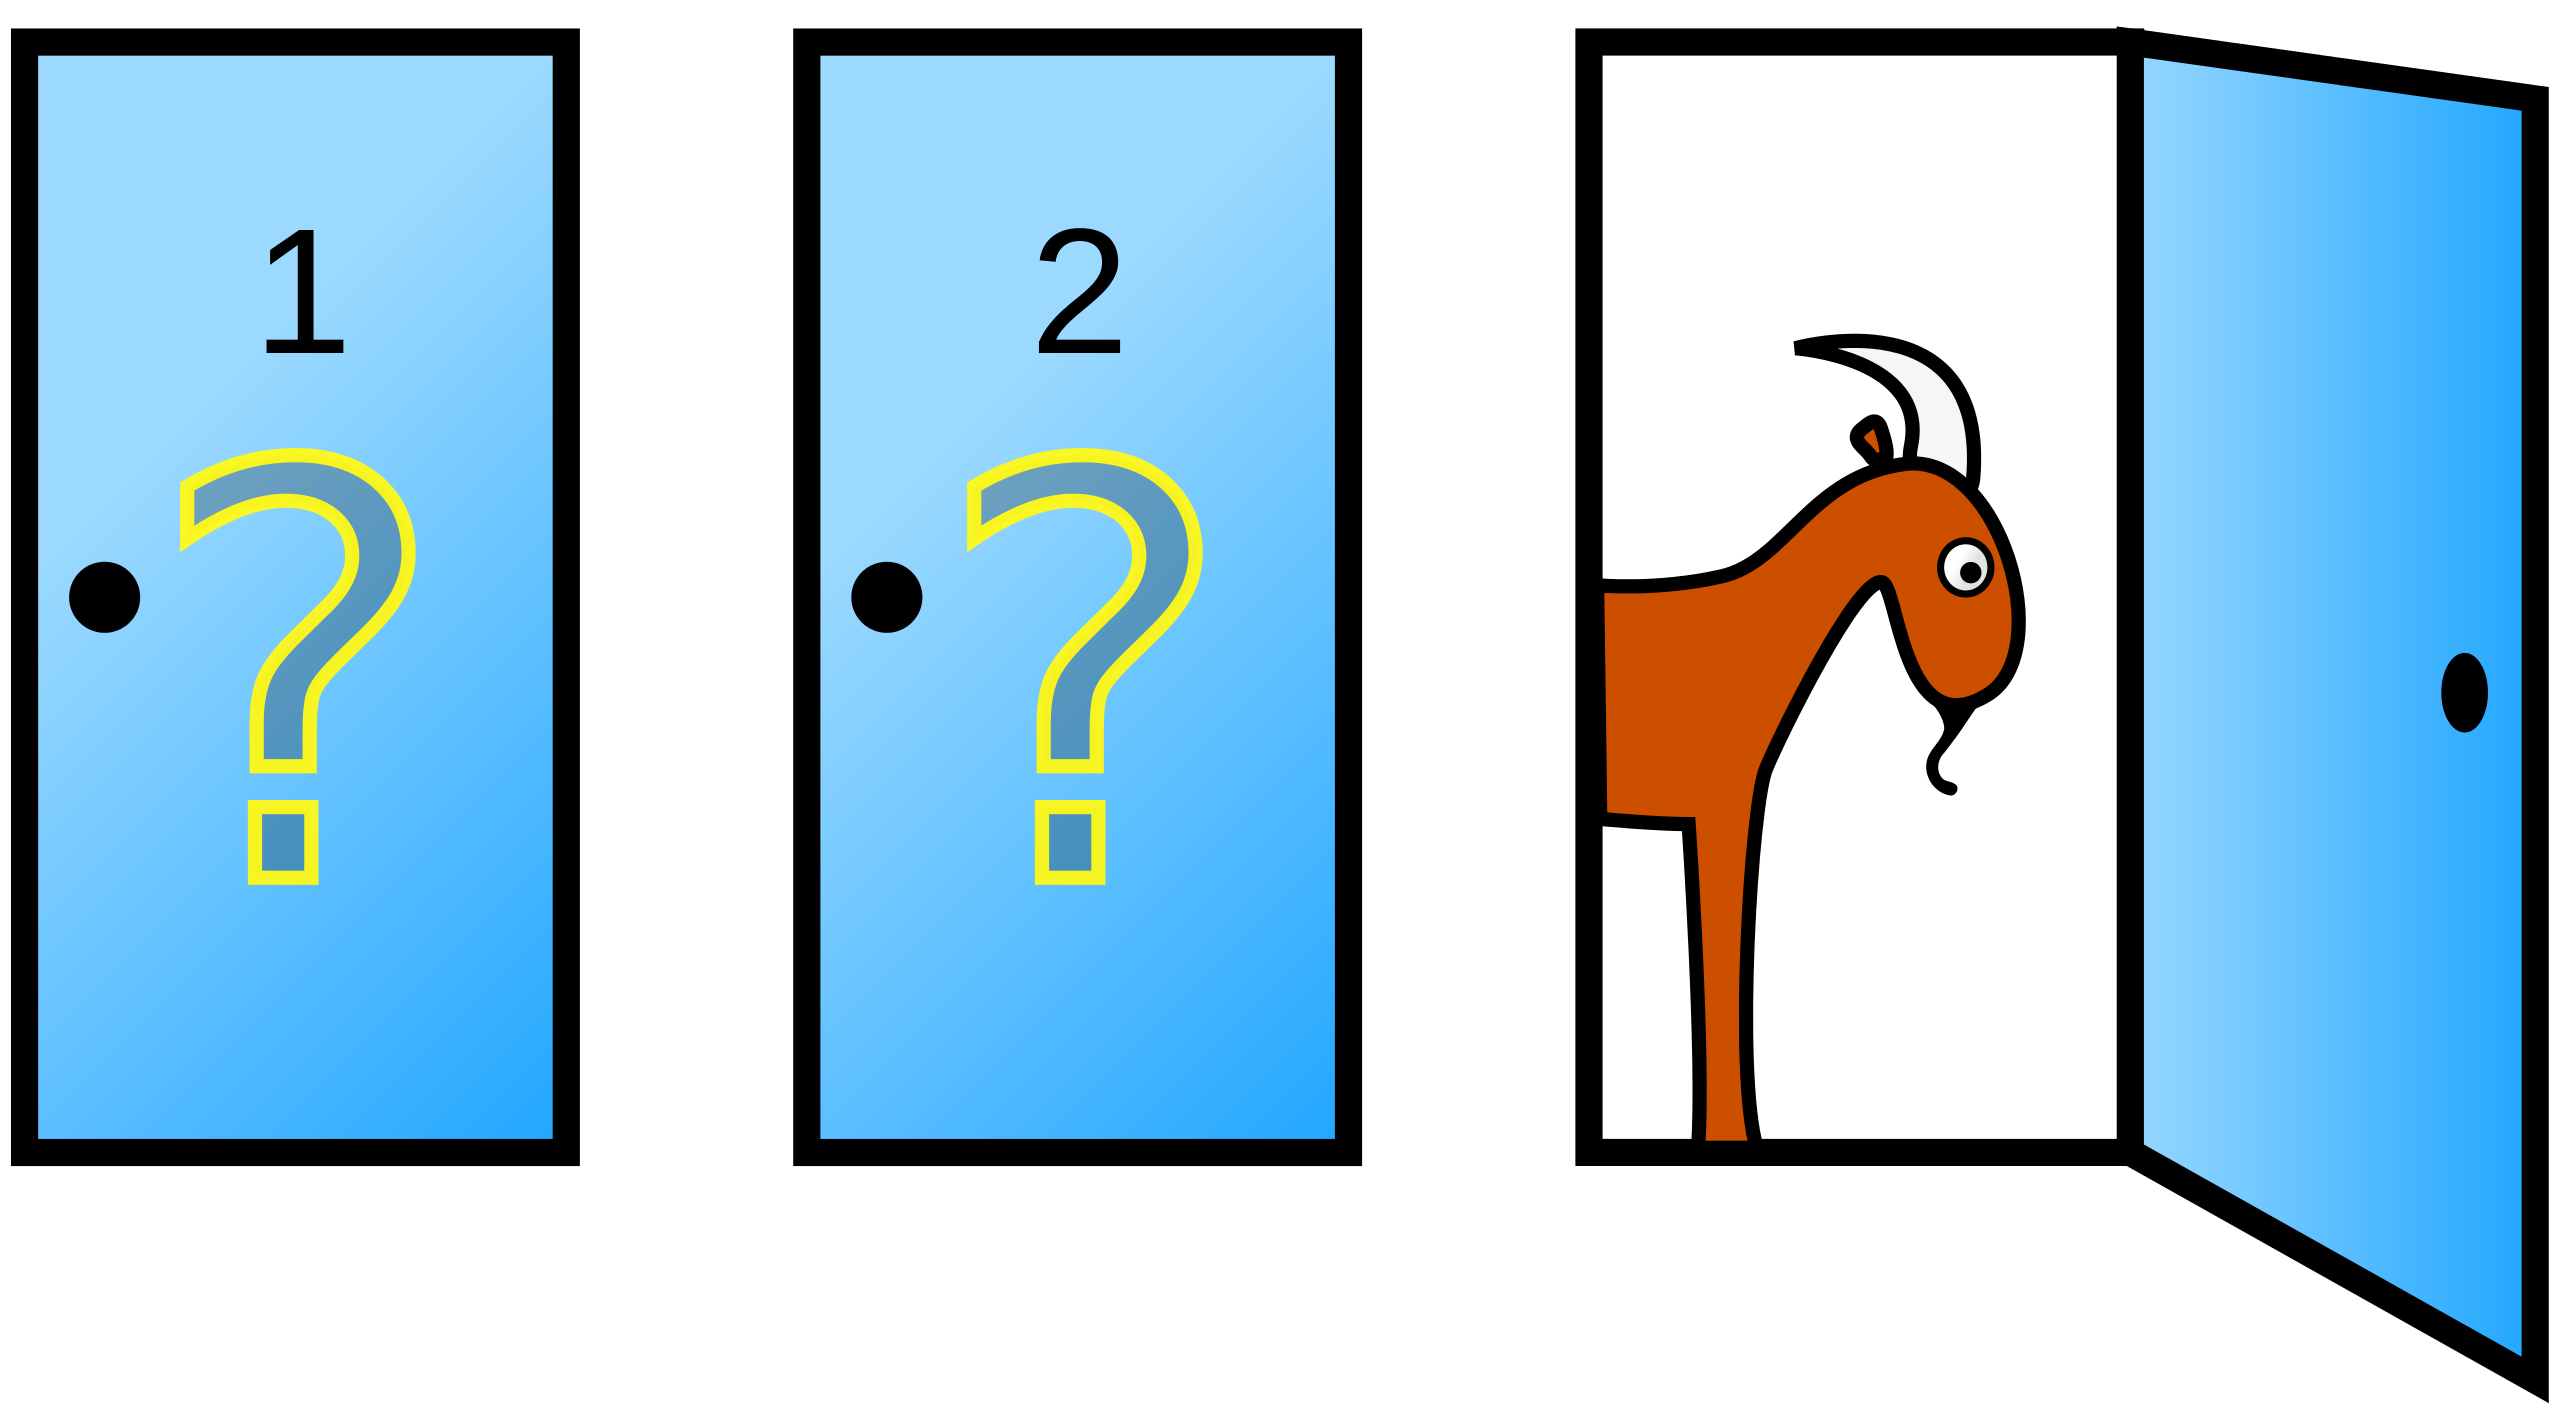
\includegraphics[height = 3cm]{images/monty_hall.png}
    \end{center}
    {\bf Q:} Do you want to switch your choice to door \#2?\\
    \pause
    {\bf A:} Yes! (door \#1 = 33\% car, door \#2 = 67\% car)
  \end{frame}

  \begin{frame}{Stein's Paradox (Efron and Morris, 1977)}
    As framed by Brown (2008):\\
    ~\\
    Two methods for predicting second-half batting average:
    \begin{enumerate}
      \item Use each player's first-half batting average
      \item Ignore the data and predict league average (.250) for everyone
    \end{enumerate}
    \vspace{1cm}
    {\bf Q:} Which method is more accurate?\\
    \pause
    {\bf A:} Method \#2
  \end{frame}

  \begin{frame}{{\it Thinking, Fast and Slow} (Kahneman, 2011)}
    \begin{columns}
      \begin{column}{0.4\textwidth}
    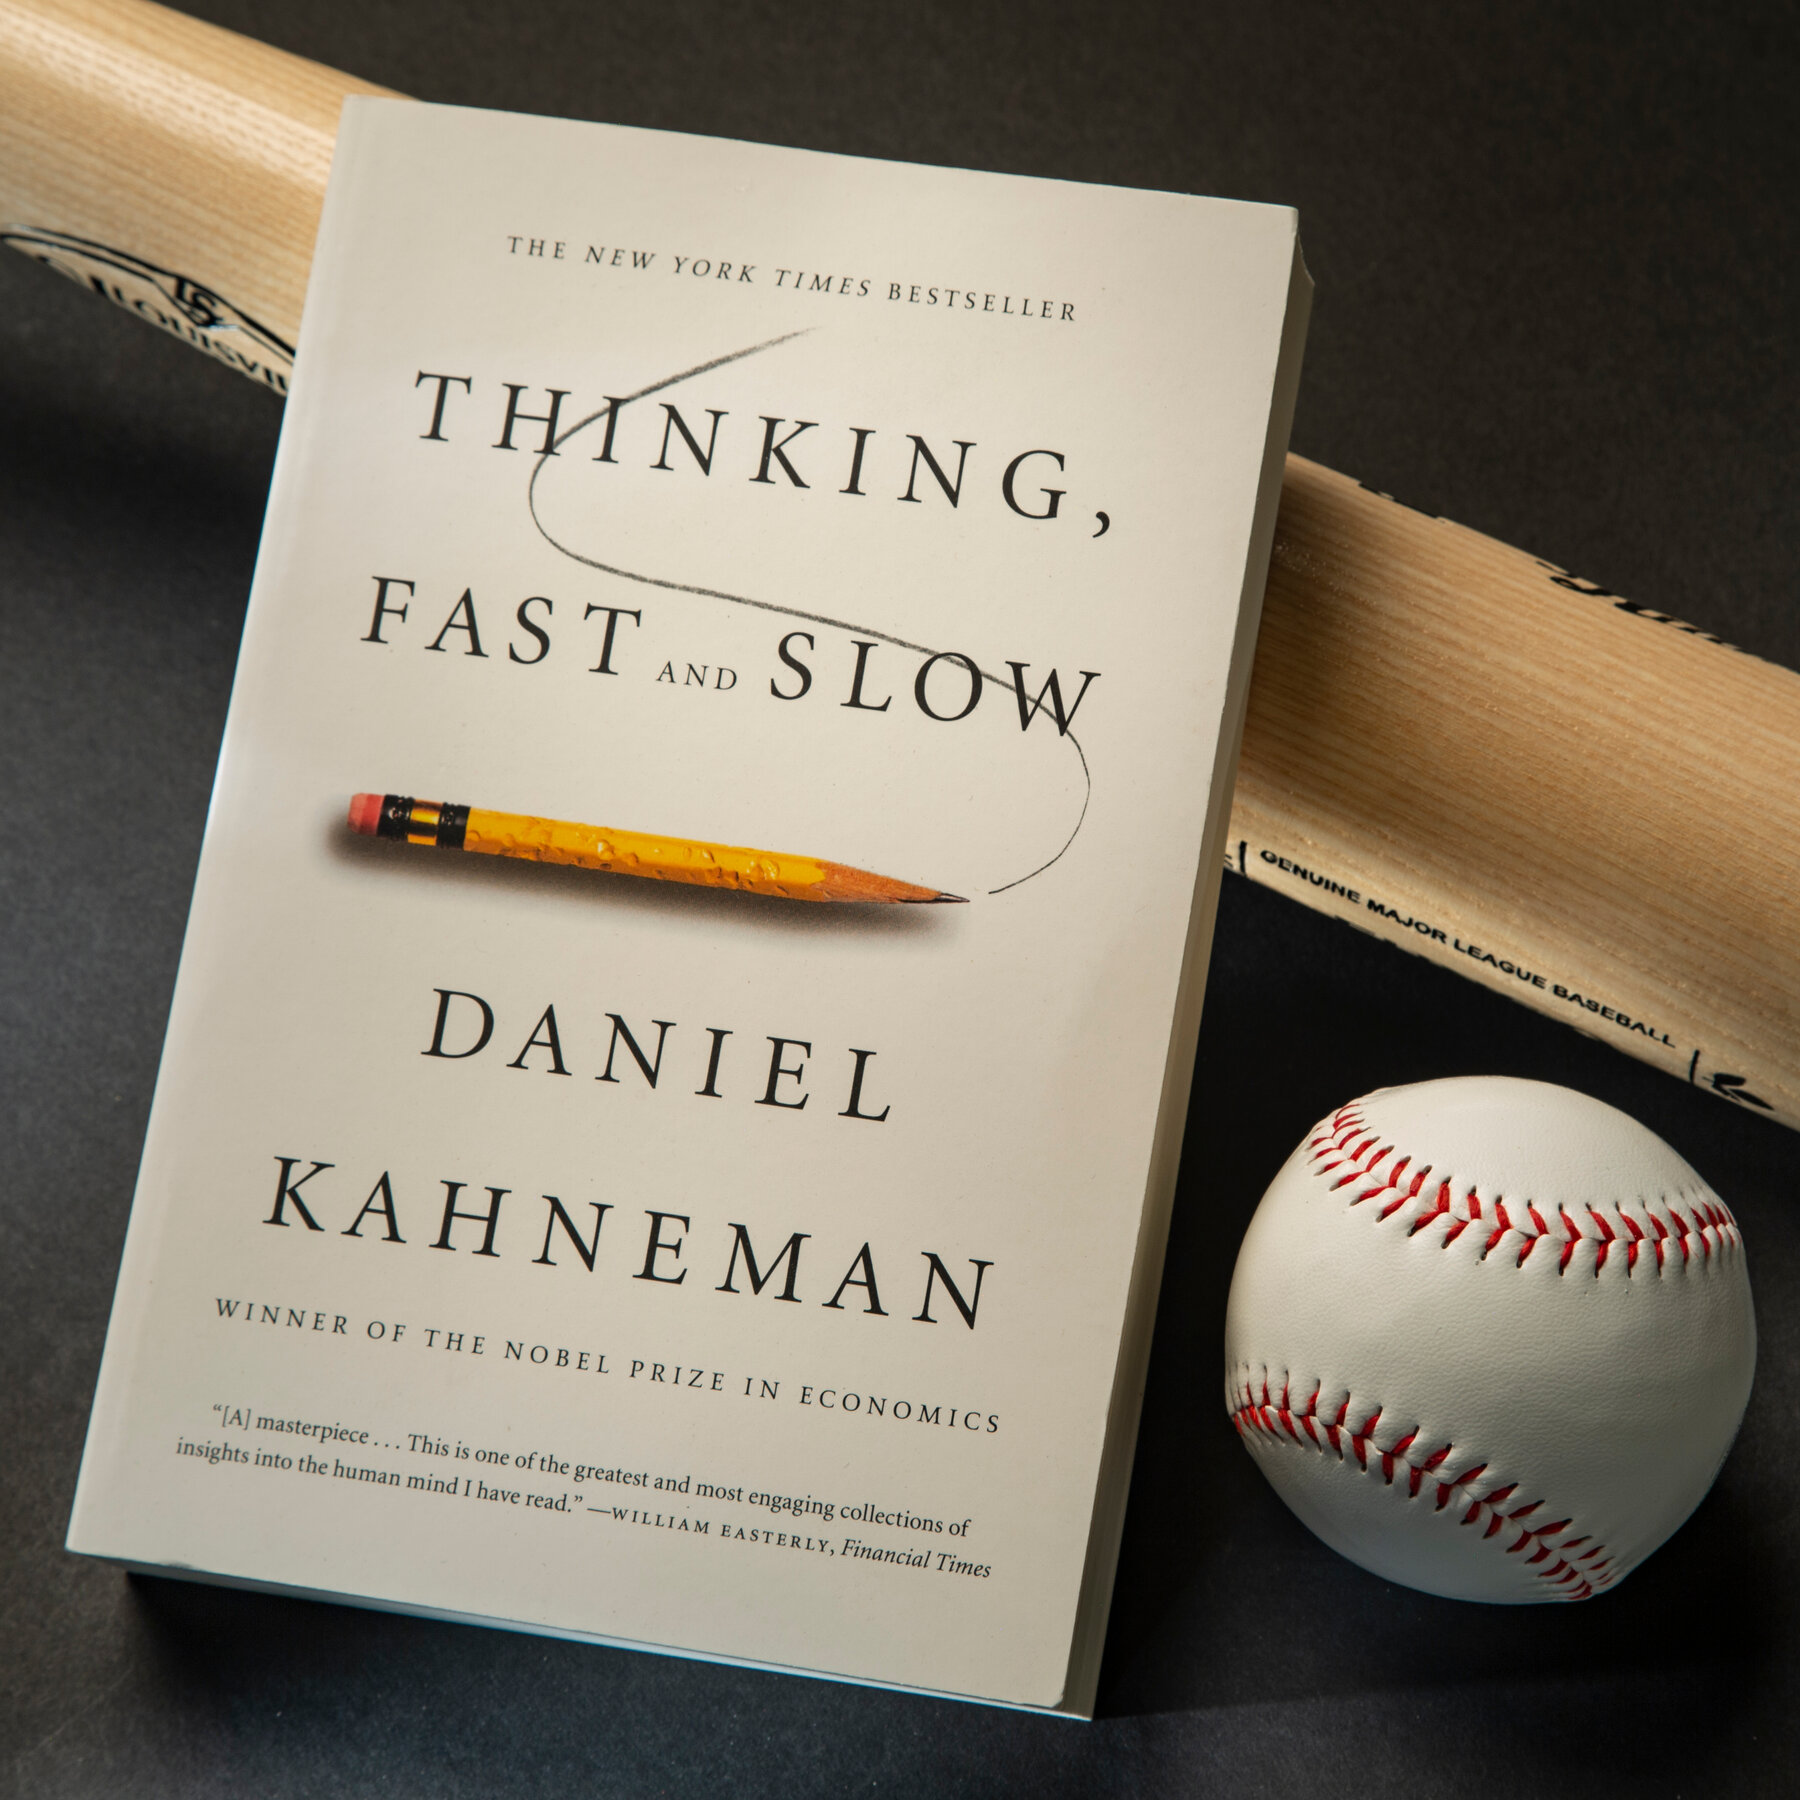
\includegraphics[width = \textwidth]{images/thinking_fast_and_slow.jpg}\\
    \small {\color{gray} \it The New York Times}
      \end{column}
      \begin{column}{0.6\textwidth}
        \begin{itemize}
          \item {\bf System 1} is fast, intuitive, emotional. {\bf System 2} is slower, more deliberative, more logical.
          \item Statistical thinking is hard because of System 1 heuristics and biases
          \item Relevant examples:
          \begin{itemize}
            \item Availability heuristic
            \item Confirmation bias
            \item Framing effect
          \end{itemize}
        \end{itemize}
      \end{column}
    \end{columns}
  \end{frame}

  \begin{frame}{The Hot Hand Fallacy (Gilovich {\it et al.}, 1985)}
    \begin{itemize}
      \item 1980-81 Philadelphia 76ers field goal data
      \begin{itemize}
        \item Shooting percentage following a make: 51\%
        \item Shooting percentage following a miss: 54\%
      \end{itemize}
      \item 1980-82 Boston Celtics free throw data
      \begin{itemize}
        \item No correlation between making 1$^{st}$ FT and making 2$^{nd}$ FT
      \end{itemize}
      \item Controlled experiment with college players (from Cornell) yielded no evidence of streaky shooting
    \end{itemize}
    ~\\
    ``Who is this guy? So he makes a study. I couldn't care less.''\\
    \hfill--- Red Auerbach\\
    ~\\
    ``The hot hand is a massive and widespread cognitive illusion.''\\
    \hfill--- Daniel Kahneman
  \end{frame}

  \begin{frame}{Takeaways (2017)}
    \begin{enumerate}
      \item Paradoxes show us that human intuition can be incorrect
      \item Human judgment can be impaired by heuristics and biases
      \item Mathematical modeling is a superior way to make decisions
    \end{enumerate}
  \end{frame}

  \begin{frame}{The Streak of Heads Paradox (Miller and Sanjurjo, 2018)}
    Flip a coin 100 times. Whenever you flip heads, write down the {\it next} outcome on a scrap of paper.\\
    ~\\
    {\bf Q:} What is the expected proportion of heads on the paper?\\
    \pause
    {\bf A:} 49.5\%\\
    ~\\
    \begin{itemize}
      \item This paradox is related to the Monty Hall problem through the ``principle of restricted choice''
      \item After adjusting Gilovich {\it et al.} (1985) for this bias, evidence supports the existence of the hot hand
    \end{itemize}
  \end{frame}

  \begin{frame}{Replication Crisis (2010s, ongoing)}
    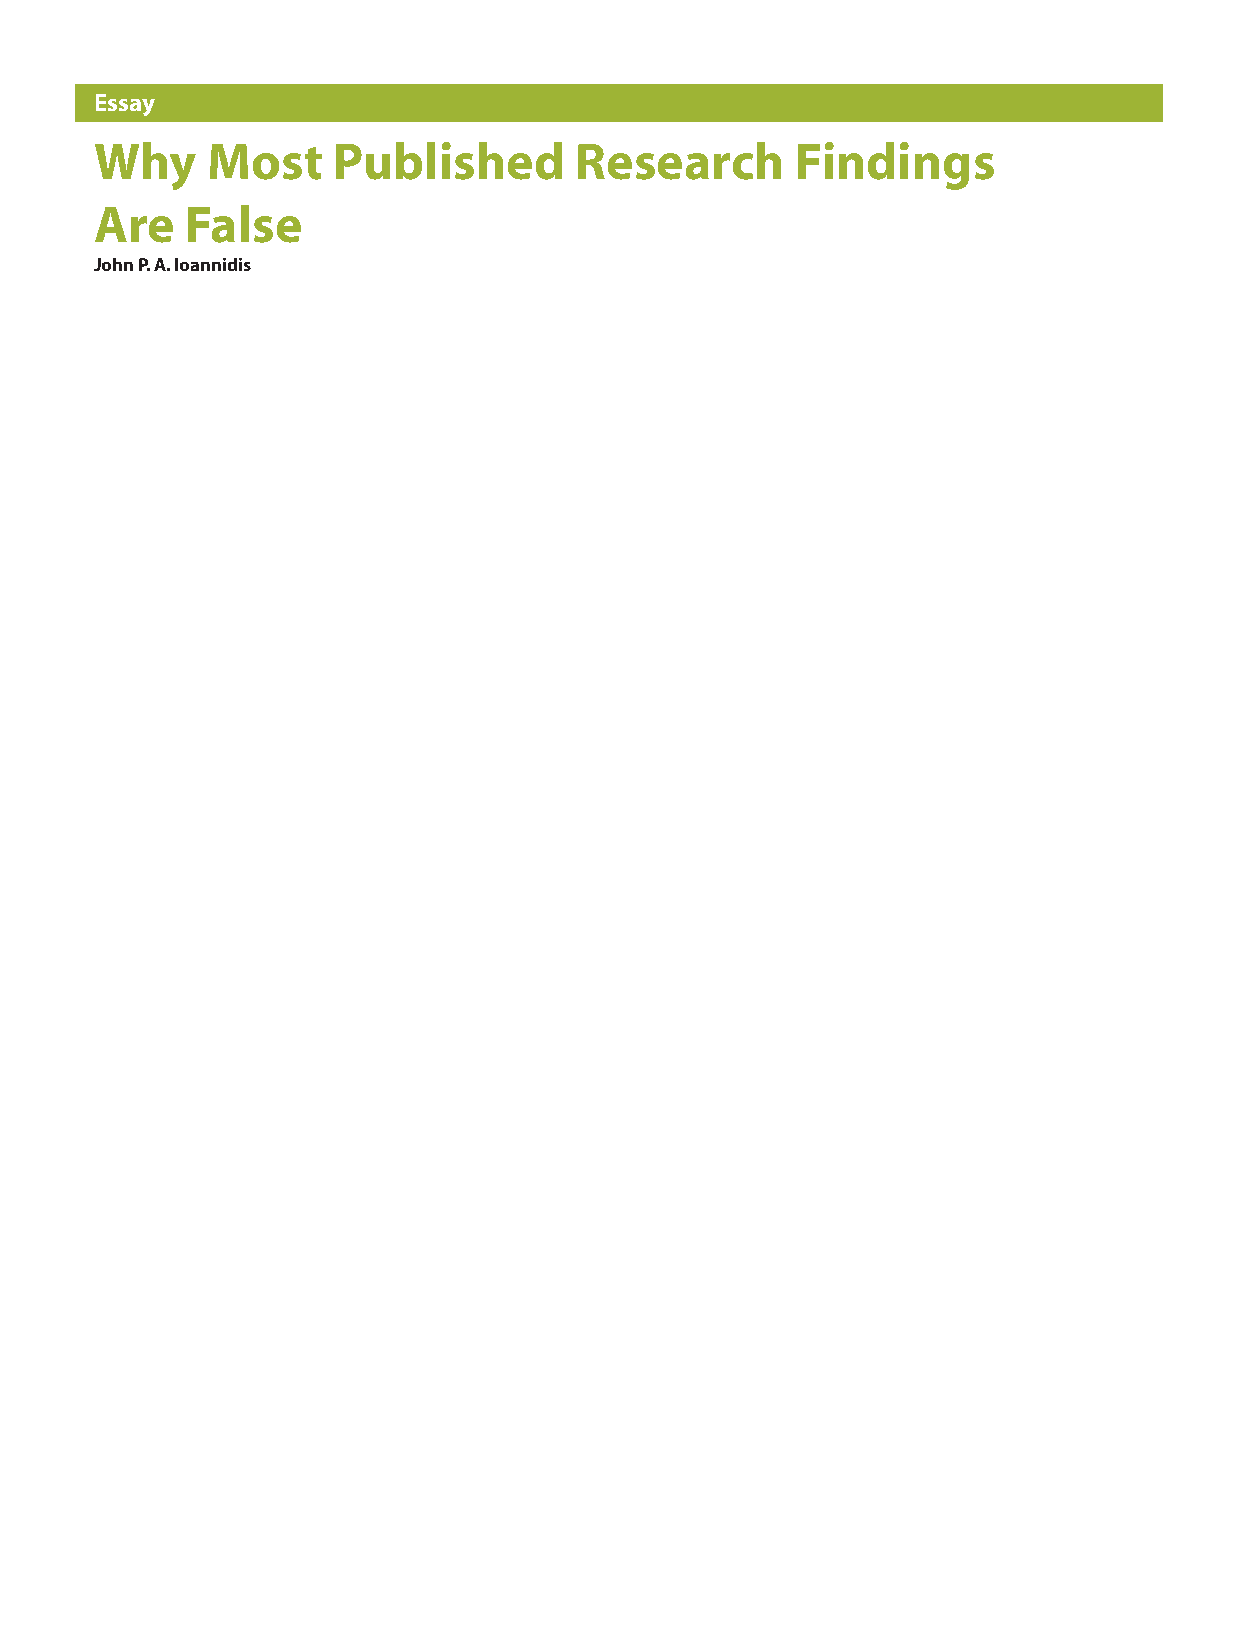
\includegraphics[width = \textwidth]{images/ioannidis.pdf}
    \begin{itemize}
      \item Because of selection bias in scientific publications,\\ many research findings fail to be replicated
      \item Shimmack (2020) estimated that only half of the results\\ cited in {\it Thinking, Fast and Slow} would be replicated
    \end{itemize}
    ~\\
    ``Readers of {\it Thinking, Fast and Slow} should read the book as a subjective account by an eminent psychologists, rather than an objective summary of scientific evidence.''\\
    \hfill--- Ulrich Schimmack
  \end{frame}

  \begin{frame}{{\it Escape from Model Land} (Thompson, 2022)}
    \begin{columns}
      \begin{column}{0.6\textwidth}
        \begin{itemize}
          \item All models make assumptions that are not literally true in real life
          \item Escaping from Model Land means validating adequacy-for-purpose
          \item Functionality as a tool to aid thinking can be more important than predictive accuracy
        \end{itemize}
      \end{column}
      \begin{column}{0.3\textwidth}
        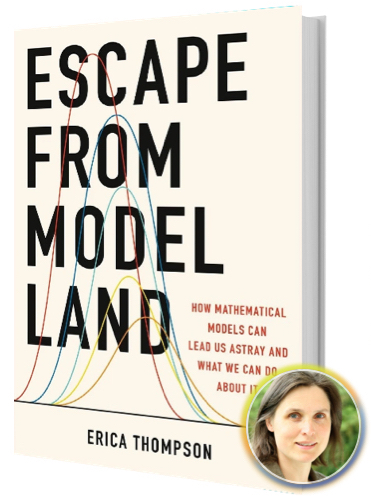
\includegraphics[height = 4cm]{images/escape_from_model_land.jpg}
      \end{column}
    \end{columns}
  \end{frame}

  \begin{frame}{Takeaways (2024)}
    \begin{enumerate}
      \item \sout{Paradoxes show us that human intuition can be incorrect}
      \item \sout{Human judgment is impaired by heuristics and biases}
      \item \sout{Mathematical modeling is a superior way to make decisions}
    \end{enumerate}
    \pause
    \begin{enumerate}
      \item We can make mistakes when applying math, too
      \item Be careful spending too much time and energy in Model Land
      \item Validation is king
    \end{enumerate}
  \end{frame}

  \begin{frame}{References}
    \tiny
    {\bf von Mises R (1939)} ``\"{U}ber aufteilungs- und besetzungswahrscheinlichkeiten''\\
    ~\\
    {\bf Simpson EH (1951)} ``The interpretation of interaction in contingency tables'' {\it Journal of the Royal Statistical Society: Series B} 13(2), 238-241.\\
    ~\\
    {\bf Stein C (1956)} ``Inadmissibility of the usual estimator for the mean of a multivariate normal distribution'' {\it Proceedings of the Third Berkeley Symposium on Mathematical Statistics and Probability} 3, 197-207.\\
    ~\\
    {\bf Selvin S (1975)} ``A problem in probability'' {\it The American Statistician} 29(1).\\
    ~\\
    {\bf Efron B and Morris C (1977)} ``Stein's paradox in statistics'' {\it Scientific American} 236(5), 119-127.\\
    ~\\
    {\bf Gilovich T, Vallone R and Tversky A (1985)} ``The hot hand in basketball: On the misperception of random sequences'' {\it Cognitive Psychology} 17(3), 295-314.\\
    ~\\
    {\bf Ioannidis JP (2005)} ``Why most published research findings are false'' {\it PLoS medicine} 2(8), e124.\\
    ~\\
    {\bf Brown LD (2008)} ``In-season prediction of batting averages: A field test of empirical Bayes and Bayes methodologies'' {\it The Annals of Applied Statistics}, 113-152.\\
    ~\\
    {\bf Kahneman D (2011)} {\it Thinking, Fast and Slow}\\
    ~\\
    {\bf Miller JB and Sanjurjo A (2018)} ``Surprised by the hot hand fallacy? A truth in the law of small numbers'' {\it Econometrica} 86(6), 2019-2047.\\
    ~\\
    {\bf Schimmack U (2020)} ``A meta-scientific perspective on Thinking: Fast and Slow'' https://replicationindex.com/2020/12/30/a-meta-scientific-perspective-on-thinking-fast-and-slow/\\
    ~\\
    {\bf Lemire J (2021)} ``This book is not about baseball. But baseball teams swear by it.'' https://www.nytimes.com/2021/02/24/sports/baseball/thinking-fast-and-slow-book.html\\
    ~\\
    {\bf Thompson E (2022)} {\it Escape from Model Land}\\
  \end{frame}

\end{document}